% BEGIN LICENSE BLOCK
% Version: CMPL 1.1
%
% The contents of this file are subject to the Cisco-style Mozilla Public
% License Version 1.1 (the "License"); you may not use this file except
% in compliance with the License.  You may obtain a copy of the License
% at www.eclipse-clp.org/license.
% 
% Software distributed under the License is distributed on an "AS IS"
% basis, WITHOUT WARRANTY OF ANY KIND, either express or implied.  See
% the License for the specific language governing rights and limitations
% under the License. 
% 
% The Original Code is  The ECLiPSe Constraint Logic Programming System. 
% The Initial Developer of the Original Code is  Cisco Systems, Inc. 
% Portions created by the Initial Developer are
% Copyright (C) 2006 Cisco Systems, Inc.  All Rights Reserved.
% 
% Contributor(s): 
% 
% END LICENSE BLOCK

\chapter{The Eplex Library}
\label{chapeplex}
%HEVEA\cutdef[1]{section}

\section{Introduction}

The eplex library allows an external Mathematical Programming solver to be
used by {\eclipse}. It is designed to allow the external solver to be seen
as another solver for {\eclipse}, possibly in co-operation with
the existing `native' solvers of {\eclipse} such as the {\it ic\/} solver. It is
not specific to a given external solver, with the differences between
different solvers (largely) hidden from the user, so that the user can
write the same code and it will run on the different solvers.

The exact types of problems that can be solved (and methods to solve them)
are solver dependent, but currently linear programming, mixed integer
programming and quadratic programming problems can be solved.

The rest of this chapter is organised as follows: the remainder of this
introduction gives a very brief description of Mathematical Programming, which
can be skipped if the reader is familiar with the concepts. 
Section~\ref{mpmodelling} demonstrates the modelling of an MP problem, and the
following section discusses some of the more advanced features of the library
that are useful for hybrid techniques.

\subsection{What is Mathematical Programming?}
\label{whatmp}

\index{Mathematical Programming (MP)}
\index{Linear Programming (LP)}
\index{Mixed Integer Programming (MIP)}
\index{optimisation (numerical)}
\index{objective function}

Mathematical Programming (MP) (also known as numerical optimisation) is the study of optimisation using
mathematical/numerical techniques. A problem is modelled
by a set of simultaneous equations: an
objective function that is to be minimised or maximised, subject to a set of
constraints on the problem variables, expressed as equalities and
inequalities. 

Many subclasses of MP problems have found important practical
applications. In particular, Linear Programming (LP)
problems and Mixed Integer Programming (MIP) problems are perhaps the most
important. LP problems have both a linear objective function and linear
constraints.  MIP problems are LP problems where some or all of the
variables are constrained to take on only integer values. 

It is beyond the scope of this chapter to cover MP in
any more detail. However, for most usages of the eplex library, the user
need not know the details of MP -- it can be treated as a black-box
solver.

\See{For more information on Mathematical Programming, you can read a
textbook on the subject such as H.~P.~Williams'  {\it Model Building in
Mathematical Programming} \cite{Williams99}.}

\quickref{Classification of MP problems}{

\begin{itemize}
\item Linear Programming (LP) problems: linear constraints and objective
function, continuous variables.
\item Mixed Integer Programming (MIP) problems: LP problems with some or
all variables restricted to taking integral values.
\end{itemize}

}

\subsection{Why interface to Mathematical Programming solvers?}
\label{whymp}

Much research effort has been devoted to developing efficient ways of
solving the various subclasses of MP problems for over 50 years. The
external solvers are state-of-the-art implementations of some of these
techniques. The eplex library allows the user to model an MP problem in
ECLiPSe, and then solve the problem using the best available MP tools.

In addition, the eplex library allows for the user to write programs that
combines MP's global algorithmic solving techniques with the local
propagation techniques of Constraint Logic
Programming. 

\subsection{Example formulation of an MP Problem} 
\begin{figure}
\begin{center}
\resizebox{0.5\textwidth}{!}{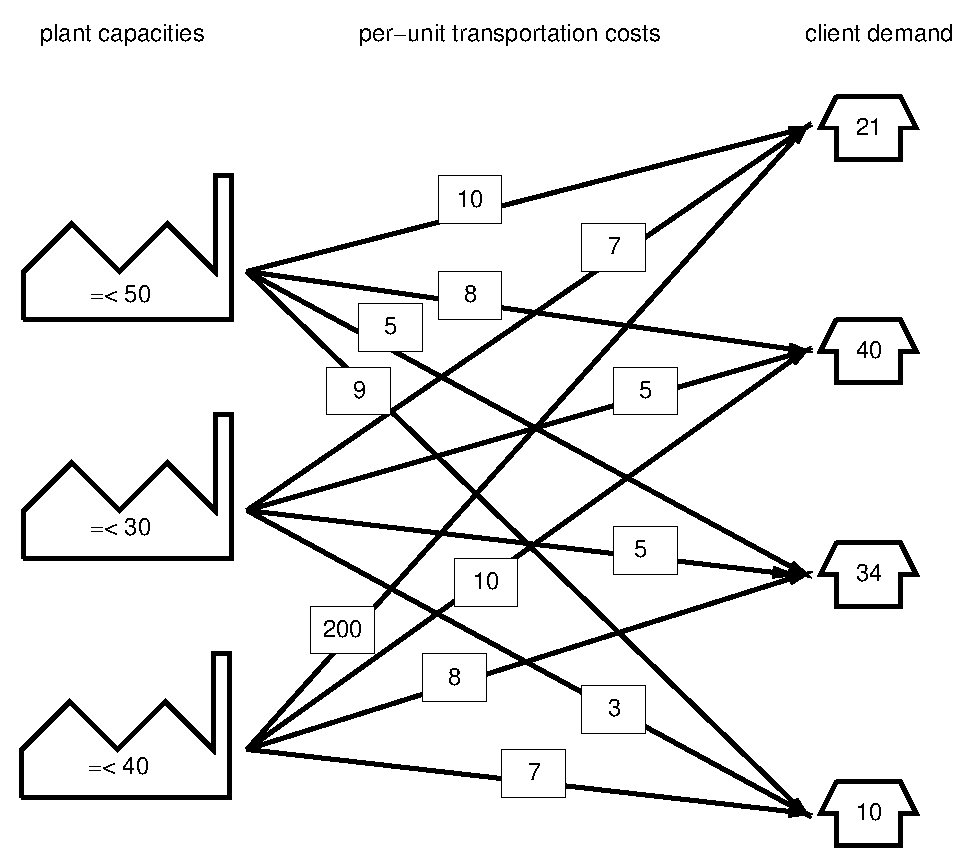
\includegraphics{tpprob.ps}}
\end{center}
\caption{An Example MP Problem}
\label{tpprob}
\end{figure}

Figure~\ref{tpprob} shows an example of an MP problem.
It is a transportation problem where 
several plants (1-3) have varying product producing capacities that must
be transported to various clients (A-D), each requiring various amounts of
the product. The per-unit cost of transporting the product to
the clients also varies. The problem is to minimise the transportation
cost whilst satisfying the demands of the clients. 

To formulate the problem, we define the amount of product transported from
a plant $N$ to a client $p$ as the variable $Np$, e.g.\ $A1$
represents the cost of transporting to plant $A$ from client $1$. There are
two kinds of constraints:

\begin{itemize}
\item The amount of product delivered from all the plants to a client must be equal to the
client's demand, e.g.\ for client A, which can recieve products from plants
1-3: \( A1 + A2 + A3 = 21 \)


\item The amount of product sent by a plant must not be more than its
capacity, e.g. for plant 1, which can send products to plants A-D:
\(A1 + B1 + C1 + D1 \leq 50 \)

\end{itemize}

The objective is to minimise the transportation cost, thus the objective
function is to minimise the combined costs of transporting the product to
all 4 clients from the 3 plants.


Putting everything
together, we have the following formulation of the problem:

Objective function:
{\small
\[
\min (10A1 + 7A2 + 200A3 + 8B1 + 5B2 + 10B3 + 5C1 + 5C2 + 8C3 + 9D1 + 3D2 + 7D3) 
\]
}

Constraints:

\begin{eqnarray*}
A1 + A2 + A3 & = & 21\\
B1 + B2 + B3 & = & 40\\
C1 + C2 + C3 & = & 34\\
D1 + D2 + D3 & = & 10\\
A1 + B1 + C1 + D1 & \leq & 50\\
A2 + B2 + C2 + D2 & \leq & 30\\
A3 + B3 + C3 + D3 & \leq & 40\\
\end{eqnarray*}

\section{How to load the library}

To use the library, you must have an MP solver that eplex can use 
(for example,
XPRESS-MP or CPLEX). Your {\eclipse} should be configured to load in a
`default' solver if there is more than one available. 

\See{See the library
manual's Eplex chapter for details for how to install the solver.} 

When configured properly, the library can be loaded with the directive:

\begin{code}
:- lib(eplex).
\end{code}

\noindent
This will load the library with the default external MP solver.

You may need a valid license in order to use an external solver. With your
{\eclipse} license, you can obtain a full OEM version of
XPRESS-MP\footnote{XPRESS-MP is a product from Dash Associates
Ltd. (www.dashoptimization.com)} that
runs with {\eclipse} version 5.5 and later from {\eclipse}'s ftp site.

\section{Modelling MP problems in {\eclipse}}
\label{mpmodelling}

\subsection{Eplex instance}

The simplest way to model an eplex problem is through an {\it eplex
instance}. Abstractly, it can be viewed as a solver module that is
dedicated to one MP problem. MP constraints can be posted to the instance 
and the problem solved with respect to an objective function by the
external solver.

Declaratively, an eplex instance can be
seen as a compound constraint consisting of all the variables and
constraints of its eplex problem. Like normal constraints, different eplex
instances can share variables, although the individual MP constraints in
an eplex instance do not necessarily have to be consistent with those in
another. 

\quickref{Eplex Instance}{

An {\bf eplex instance} represents a single MP problem in a
module. Constraints for the problem are posted to the module. The
problem is solved with respect to an objective function.
}

\subsection{Example modelling of an MP problem in {\eclipse}}

\index{modelling, LP problem}
The following code models (and solves) the transportation problem of
Figure~\ref{tpprob}, using an eplex instance:

{\small
\begin{code}
:- lib(eplex).

:- eplex_instance(prob).  % a. declare an eplex instance

main1(Cost, Vars) :-
        % b. create the problem variables and set their range
        Vars = [A1,A2,A3,B1,B2,B3,C1,C2,C3,D1,D2,D3], 
        prob: (Vars \$:: 0.0..1.0Inf),

        % c. post the constraints for the problem to the eplex instance
        prob: (A1 + A2 + A3 \$= 21),
        prob: (B1 + B2 + B3 \$= 40),
        prob: (C1 + C2 + C3 \$= 34),
        prob: (D1 + D2 + D3 \$= 10),

        prob: (A1 + B1 + C1 + D1 \$=< 50),
        prob: (A2 + B2 + C2 + D2 \$=< 30),
        prob: (A3 + B3 + C3 + D3 \$=< 40),

        % d. set up the external solver with the objective function
        prob: eplex_solver_setup(min(
                10*A1 + 7*A2 + 200*A3 + 
                 8*B1 + 5*B2 + 10*B3 +
                 5*C1 + 5*C2 +  8*C3 + 
                 9*D1 + 3*D2 +  7*D3)),

        %------------------------------- End of Modelling code

        prob: eplex_solve(Cost).  % e. Solve problem using external solver

\end{code}
}

To use an eplex instance, it must first be declared with \verb'eplex_instance/1'. 
This is usually done with a directive, as in line \verb'a'.
Once
declared, an eplex instance can be referred to using its name like a module
qualifier.

We first create the problem
variables and set their range to be non-negative, as is conventional in MP.
Note that the bounds are posted to our eplex instance, using \verb'$::/2'.
\Note{The default bounds for variables is -1.0Inf..1.0Inf. Bounds posted to
  an eplex instance are specific to that eplex instance.}

Next, we set up the MP constraints for the
problem by posting them to the eplex instance. 
The MP constraints accepted by eplex are the arithmetic equalities and 
inequalities:
\verb'$=/2', \verb'$=</2' and \verb'$>=/2'.
\Note{The arithmetic constraints can be linear expressions on both
sides. The restriction to linear
expressions originates from the external solver.}
\index{\$=/2!eplex}
\index{\$>=/2!eplex}
\index{\$=</2!eplex}
\index{eplex\_solver\_setup/1}
\index{eplex\_instance/1}
\index{eplex\_solve/1}

We need to setup the external solver with the eplex instance, so
that the problem can be solved by the external solver. This is done by
\verb'eplex_solver_setup/1', with the objective
function given as the argument, enclosed by either \verb'min(...)' or \verb'max(...)'. In this case, we are minimising.
Note that
generally the setup of the solver and the posting of the MP constraints can be
done in any order.

Having set up the problem, we can solve it
by calling \verb'eplex_solve/1' in line \verb'e'. 

When an instance gets solved, the external solver takes into account all
constraints posted to that instance, the current variable bounds for the
problem variables, and the objective specified during setup.

In this case, there is an optimal solution of 710.0:

\begin{quote}\begin{verbatim}
?-  main1(Cost, Vars).

Cost = 710.0
Vars = [A1{0.0 .. 1e+20 @ 0.0}, A2{0.0 .. 1e+20 @ 21.0}, ....]
\end{verbatim}\end{quote}
Note that the problem variables are not
instantiated by the solver. However, the `solution' values, i.e.\ the
values that the variable are given by the solver, are available in the
eplex attribute. The eplex attribute is shown as \verb'Lo..Hi @ Sol' where
\verb'Lo' is the lower bound, \verb'Hi' the upper bound, and \verb'Sol' the
solution value for the variable (e.g., \verb'A2' has the solution value of
21.0 in the example above). Note also that the external solver may not
allow very large floats, hence \verb'1e+20', this external solver's
representation of infinity, is the upper bound of the
variables, even though we specified \verb'1.0Inf' in our code. 

One reason the problem variables are not assigned their solution values is
so that the eplex problem can be solved again, after it has been modified.
A problem can be modified by the addition of more constraints, and/or
changes in the bounds of the problem variables.

\subsection{Getting more solution information from the solver}

The solution values of the problem variables can be obtained by
\verb'eplex_var_get/3'. The example program in the
previous section can be modified to return the solution values:

{\small
\begin{code}
main2(Cost, Vars) :-
        ....  % same as previous example up to line e
        prob: eplex_solve(Cost),  % e. Solve problem using external solver
        (foreach(V, Vars) do
            % f. set the problem variables to their solution values
            prob: eplex_var_get(V, typed_solution, V) 
        ).
\end{code}}
\index{eplex_var_get/3}

In line \verb'f', \verb'eplex_var_get/3' is used to obtain the solution
value for a problem variable. The second argument, set to \verb'typed_solution', 
 specifies that we want the solution value for the variable to be returned.
Here, we instantiate the problem variable itself to the solution value
with the third argument:

\begin{quote}\begin{verbatim}
?- main2(Cost, Vars).


Cost = 710.0
Vars = [0.0, 21.0, 0.0, 16.0, 9.0, 15.0, 34.0, 0.0, 0.0, 0.0, 0.0, 10.0]
\end{verbatim}\end{quote}

Note that, in general, an MP problem can have many optimal solutions, i.e.\
different solutions which give the optimal value for the objective function.
As a result, the above
instantiations for \verb'Vars' might not be what is returned by the solver
used.


\subsection{Adding integrality constraints}
\index{modelling, MIP}

In general, a problem variable is not restricted to taking integer
values. However, for some problems, there may be a requirement that some or
all of the variable values be strictly integral (for example, in the previous
transportation problem, it may be that only whole units of the
products can be transported; also variables may often be used to model
booleans by allowing them to take on the values of 0 or 1 only). 
This can be specified  by
posting an additional \verb'integers/1' constraint on the
variables. 

\index{integers/1!eplex}
Consider the example problem again, where it so happens that the
optimal value for the objective function can be satisfied with integral
values for the variables. To show the differences
that imposing integer constraints might make, we add the constraint that
client A must receive an equal amount of products from plants 1 and 2. Now
the problem (without the integer constraints) can be written as:

{\small
\begin{code}
:- lib(eplex).

:- eplex_instance(prob).  

main3(Cost, Vars) :-
        Vars = [A1,A2,A3,B1,B2,B3,C1,C2,C3,D1,D2,D3], 
        prob: (Vars \$:: 0.0..1.0Inf),
        prob: (A1 + A2 + A3 \$= 21),
        prob: (B1 + B2 + B3 \$= 40),
        prob: (C1 + C2 + C3 \$= 34),
        prob: (D1 + D2 + D3 \$= 10),

        prob: (A1 + B1 + C1 + D1 \$=< 50),
        prob: (A2 + B2 + C2 + D2 \$=< 30),
        prob: (A3 + B3 + C3 + D3 \$=< 40),

        prob: eplex_solver_setup(min(
                10*A1 + 7*A2 + 200*A3 + 
                 8*B1 + 5*B2 + 10*B3 +
                 5*C1 + 5*C2 +  8*C3 + 
                 9*D1 + 3*D2 +  7*D3)),

        prob: (A1 \$= A2), % g. the new constraint, added after setup

        %------------------------------- End of Modelling code

        prob: eplex_solve(Cost),  
        (foreach(V, Vars) do
            prob: eplex_var_get(V, typed_solution, V) 
        ).
\end{code}}

In this example, the new constraint in line \verb'g' is imposed after the
solver setup. In fact it can be imposed anytime before
\verb'eplex_solve(Cost)' is called.

This problem also has an optimal \verb'Cost' of 710, the same as the original
problem. However, the solution values are not integral:

\begin{quote}\begin{verbatim}
?- main3(Cost, Vars).

Cost = 710.0
Vars = [10.5, 10.5, 0.0, 5.5, 19.5, 15.0, 34.0, 0.0, 0.0, 0.0, 0.0, 10.0]
\end{verbatim}\end{quote}

Now, to impose the constraints that only whole units of the products can be
transported, we modify the program as follows:

{\small
\begin{code}
main4(Cost, Vars) :-
        Vars = [A1,A2,A3,B1,B2,B3,C1,C2,C3,D1,D2,D3], 
        prob: (Vars \$:: 0.0..1.0Inf),
        prob: integers(Vars),  % h. impose the integrality constraint
        ....% Rest is the same as main3
\end{code}}

In line \verb'h', we added the \verb'integers/1' constraint. This imposes
the integrality constraint on \verb'Vars' for the eplex instance
\verb'prob'. Now,
the external solver will only assign integer solution values to the
variables in the list. \Note{In fact, with the integer
constraints, the problem is solved
as a MIP problem rather than an LP problem, which involves different
(and generally computationally more expensive) techniques. This difference
is hidden from the eplex user.}

Running this program, we get:

\begin{quote}\begin{verbatim}

?- main4(Cost,Vars).

Cost = 898.0
Vars = [10, 10, 1, 6, 20, 14, 34, 0, 0, 0, 0, 10]

\end{verbatim}\end{quote}

In this case, \verb'A1' and \verb'A2' are now integers. In fact, notice
that all the values returned are now integers rather than floats. This is
because the  \verb'typed_solution' option of \verb'eplex_var_get/3'
returns the solution values taking into account if the variables have been
declared as integers for the eplex instance.
\Note{Posting an integers/1 constraint to an eplex instance only
  inform the external solver to treat those variables as integers (in fact
  the external solver will still represent the variables as floats, but
  will only assign intergral solution values to them), but does
  not constrain the variable itself to be of type integer.}



\quickref{Modelling an MP Problem}{
\begin{itemize}
\item Declare an eplex instance using {\bf eplex_instance(+Instance)}.
\item Post the constraints ({\bf \$=/2, \$>=/2, \$=</2, integers/1,
  \$::/2}) for the problem to the eplex instance.
\item Setup the solver with the objective function using 
\newline{\bf Instance: eplex_solver_setup(+ObjFunc)}.
\end{itemize}

}

\section{Repeated Solving of an Eplex Problem}

Part of the power of using the eplex library comes from being able to solve
an eplex problem repeatedly after modification.
For example, we can solve the original transportation
problem, add the extra constraint, and resolve the problem.
Remember that as \verb'eplex_solve/1' instantiates its argument, we
need to use a new variable for each call:

{\small
\begin{code}
        .... % setup the constraints for the original problem as before
        prob: (A3 + B3 + C3 + D3 =< 40),

        prob: eplex_solver_setup(min(....)), % as before

        prob: eplex_solve(Cost1),     % h. solve original problem
        prob: (A1 \$= A2),
        prob: eplex_solve(Cost2),     % i. solve modified problem
        .....
\end{code}}

Note that posted constraints behave logically: they are added to an eplex
instance when posted, and removed when they are backtracked over.

In the examples so far, the solver has been invoked explicitly.
However, the solver can also behave like a normal constraint, i.e.\ it is
automatically invoked when certain conditions are met. 

As an example, we implement the standard branch-and-bound method of
solving a MIP problem, using the external solver as an LP solver only.
Firstly we outline how this can be
implemented with the facilities we have already encountered. We then show
how this can be improved usin more advanced features of \texttt{lib(eplex)}.

With the branch-and-bound approach, a search-tree is formed, and at each node a
`relaxed' version of the MIP problem is solved as an LP problem.
Starting at the root, the problem solved is the original MIP problem, but
without any of the integrality constraints:
{\small
\begin{code}
:- eplex_instance(mip).

main5(Cost, Vars) :-
      % set up variables and constraints, but no integers/1 constraints
      ....
      % assume minimise for simplicity
      mip: eplex_solver_setup(min(Obj)), 
      mip: eplex_solve(RelaxedCost),
      mip: (Cost \$>= RelaxedCost),  % RelaxedCost is lower bound 
\end{code}}
\begin{figure}
\begin{center}
\resizebox{0.35\textwidth}{!}{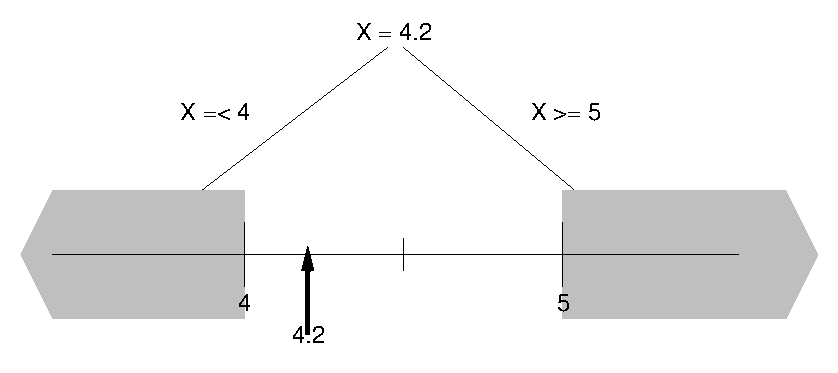
\includegraphics{mipnode.ps}}
\end{center}
\caption{Labelling a variable at a MIP tree node}
\label{mipnode}
\end{figure}
In general, this initial LP solution contains non-integer assignments
to integer variables. The objective value of this LP is a lower bound on
the actual MIP objective value.
The task of the search is to find integer assignments
for the integer variables that optimises the objective function. 
Each node of the
search-tree solves the problem with extra bound constraints on these
variables. At each node, a particular variable is `labelled' as shown in
Figure~\ref{mipnode}. The integer variable in this case has been assigned
the non-integer value of 4.2. In the subsequent nodes of the tree, we
consider two  alternate problems, which creates two branches in the search. In one
problem, we impose the bound constraint $X \leq 4$, and in the other, $X
\geq 5$: these are the two nearest integer values to 4.2. In each branch,
the problem is  solved
again as an LP problem with its new bound for the variable:

{\small
\begin{code}
branching(IntVars) :-
      ....
      % for each integer variable X which violates the integer constraint
      mip: eplex_var_get(X, solution, XVal),
      ...
      Split is floor(XVal),
      % choice: branch on the two ranges for X
      (mip: (X \$=< Split) ; mip: (X \$>= Split + 1)),
      mip: eplex_solve(RelaxedCost),
      ...% repeat until there are no integer violations
\end{code}}

A choice-point for the two alternative branchings is created in the above
code, the problem is solved with one of the branchings (\verb'X $=< Split').
The program then proceeds to further labelling of the variables. The
alternative branch is left to be tried on backtracking.


Eventually, if the problem has a solution, all the integer
variables will be `labelled' with integer values, resulting in a solution to the
MIP problem. However, this will generally not be optimal, and so the program
needs to backtrack into the tree to search for a better solution by trying
the other branches for the variables, using the
existing solution value as a bound.
This `branch-and-bound' search technique is implemented in {\tt
lib(branch_and_bound)}.

\quickref{Reminder: use {\eclipse} libraries!}{Remember that {\eclipse} provides
libraries that make some programming tasks much easier. There is no
need to write your own code when you can use what is
provided by an {\eclipse} library.}

\begin{sloppypar}
In the code, the external solver is invoked explicitly at every node. This
however may not be necessary as the imposed bound may already be satisfied.
As stated at the start of this section, the invocation of the solver could be done in a
data-driven way, more like a normal constraint.
This is done with \verb'eplex_solver_setup/4':
\verb'eplex_solver_setup(+Obj,-ObjVal,+Options,+Trigs)', a more
powerful version of \verb'eplex_solver_setup/1' for setting up a
solver. The \verb'Trigs' argument specifies a list of `trigger
modes' for triggering the solver. \See{See the {\eclipse} reference manual for a
complete  description of the predicate.}
\end{sloppypar}

\index{eplex\_solver\_setup/4}
For our example, we add a bound constraint at each node to exclude a
fractional solution value for a variable. The criterion we want to use is
to invoke the solver only if this old solution value is excluded by the new
bounds (otherwise the external solver will solve the same problem
redundantly). This is done by
specifying \verb'deviating_bounds' in the trigger modes.
The full code that
implements a MIP solution for the
example transportation problem is given below: 
{\small
\begin{code}
:- lib(eplex).
:- lib(branch_and_bound).

:- eplex_instance(mip).

main6(Cost, Vars) :-
        % b. create the problem variables and set their range
        Vars = [A1,A2,A3,B1,B2,B3,C1,C2,C3,D1,D2,D3], 
        mip: (Vars :: 0.0..1.0Inf),

        % c. post the constraints for the problem to the eplex instance
        mip: (A1 + A2 + A3 \$= 21),
        mip: (B1 + B2 + B3 \$= 40),
        mip: (C1 + C2 + C3 \$= 34),
        mip: (D1 + D2 + D3 \$= 10),

        mip: (A1 + B1 + C1 + D1 \$=< 50),
        mip: (A2 + B2 + C2 + D2 \$=< 30),
        mip: (A3 + B3 + C3 + D3 \$=< 40),
        mip: (A1 \$= A2),

        % j. post the objective function as a constraint 
        ObjFunc = 10*A1 + 7*A2 + 200*A3 + 
                   8*B1 + 5*B2 + 10*B3 +
                   5*C1 + 5*C2 +  8*C3 + 
                   9*D1 + 3*D2 +  7*D3,
        mip: (ObjFunc  \$= Cost),

        % k. this is a more flexible method for setting up a solver.
        %    [deviating_bounds] specifies that the external solver should be
        %    invoked when any solution value is outside the variable bounds 
        mip: eplex_solver_setup(min(ObjFunc), Cost, [], [deviating_bounds]),

        % l. Use the branch_and_bound library to do the branch and bound
        bb_min(( branching(Vars), 
                 mip: eplex_get(cost, Cost)
                 (foreach(V, Vars) do mip: eplex_var_get(V,solution,V))
               ), Cost, _).

branching(IntVars) :-
        % Find a variable X which does not have an integer solution value
        (integer_violation(IntVars, X, XVal) ->
            % m. try the closer integer range first
            Split is round(XVal),
            (Split > XVal ->
                (mip: (X \$>= Split) ;  mip: (X \$=< Split - 1))
            ;
                (mip: (X \$=< Split) ; mip:  (X \$>= Split + 1))
            ),
            branching(IntVars)
        ;
            % cannot find any integer violations; found a solution
            true
        ).

% returns Var with solution value Val which violates the integer constraint
integer_violation([X|Xs], Var, Val) :-
        mip: eplex_var_get(X, solution, RelaxedSol),
        % m. we are dealing with floats here, so need some `margin' for a
        %    float value to be considered integer (1e-5 on either side)
        (abs( RelaxedSol - round(RelaxedSol) ) >= 1e-5 ->
            Var = X, Val = RelaxedSol
        ;
            integer_violation(Xs, Var, Val)
        ).

\end{code}}

The setup of the solver is done in line \verb'k', with the use of the
\verb'deviating_bounds' trigger mode. There are no explicit calls to trigger the
solver -- it is triggered automatically. In addition, the first call to
\verb'eplex_solve/1' for an initial solution
is also not required, because when trigger modes are specified, then
by default, \verb'eplex_solver_setup/4' will invoke the solver once the
problem is setup. 

\begin{sloppypar}
Besides the \verb'deviating_bounds'
trigger condition, the other argument of interest in our use of
\verb'eplex_solver_setup/4' is the second argument,
the objective value of the problem (\verb'Cost' in the example): 
recall that this was returned previously by \verb'eplex_solve/1'.
Unlike in \verb'eplex_solve/1', the variable is {\it not\/}
instantiated when the solver returns. Instead, one of the bounds (lower
bound in the case of minimise) is updated
to the optimal value, reflecting the range the objective value can take,
from suboptimal to the `best' value at optimal. The variable is therefore
made a problem variable by posting of the objective as a constraint in line
\verb'j'. This informs the external solver needs to be informed
that the \verb'Cost' variable is the objective value.

\end{sloppypar}

In line \verb'm', the branch choice is created by the posting of the bound
constraint, which may trigger the external solver. Here, we use a
simple heuristic to decide which of the two branches to try first: the
branch with the integer range closer to the relaxed solution value.
For example, in the situation of Figure~\ref{mipnode}, the branch with
\verb'X $=< 4' is tried first since the solution value of 4.2 is
closer to 4 than 5.

By using {\it lib(branch_and_bound)\/}'s \verb'bb_min/3' predicate in \verb'm',  
there is no need to explicitly write our own branch-and-bound routine. However, 
this predicate requires the cost variable to be instantiated, so we call
\verb'eplex_get(cost, Cost)' to instantiate \verb'Cost' at the end of
each labelling of the variables. We also get the solution values for the
variables, so that the branch-and-bound routine will remember it.
The final value returned in \verb'Cost' (and {\tt Vars} for the solution
values) 
is the optimal value after the branch-and-bound search, i.e.\ the
optimal value for the MIP problem.

\quickref{More advanced modelling in eplex}{
\begin{itemize}
\item Use {\bf
Instance:eplex_solver_setup(+Obj,-ObjVal,+Opts,+Trigs)} to
set up an external solver state for instance Instance. Trigs specifies a
list of trigger conditions to automatically trigger the external solver.
\item {\bf Instance:eplex_var_get(+Var,+What,-Value)} can be used to obtain
information for the variable {\bf Var} in the eplex instance.
\item {\bf Instance:eplex_get(+Item, -Value)} can be used to  retrieve
information about the eplex instance's solver state.
\end{itemize}
}
\index{eplex\_get/2}

Of course, in practice, we do not write our own MIP solver, but 
use the MIP solver provided with the external solvers instead. These
solvers are highly optimised and tightly coupled to their own LP solvers. 
The techniques of solving relaxed subproblems described here are however
very useful for combining the external solver with other solvers in a
hybrid fashion. \See{See chapter~\ref{chaphybrid} for more details on hybrid techniques.}

\section{Exercise}

A company produces two types of products T1 and T2, which requires the
following resources to produce each unit of the product:

\vspace{3mm}
\begin{center}
\begin{tabular}{|r||r|r|}\hline
Resource & T1 & T2\\ \hline
Labour (hours) & 9 & 6\\ \hline
Pumps (units) & 1 & 1\\ \hline
Tubing (m) & 12 & 16\\ \hline
\end{tabular}
\end{center}
\vspace{3mm}

The amount of profit per unit of products are:

\begin{description}
\item[T1] \pounds350
\item[T2] \pounds300
\end{description}

They have the following resources available: 1566 hours of labour, 200
pumps, and 2880 metres of tubing.



\begin{enumerate}
\item Write a program to maximise the profit for the company, using eplex
as a black box solver.   Write a predicate that returns the profit and the
    values for T1 and T2.

\item What program change is required to answer this question:
    What profit can be achieved if exactly 150 units of T1 are required?

\item What would the profit be if fractional numbers of refrigerators could
    be produced?

\item Rewrite the program from (1) without optimize/2, using
    eplex_solver_setup/1, eplex_solve/1, and eplex_var_get/3.

\item In the program from (4), remove the integrality constraints (so that eplex
    only sees an LP problem).  Solve the integer problem by interleaving
    solving of the LP problem with a rounding heuristic:

\begin{itemize}
    \item solve the continuous relaxation
    \item round the solution for T1 to the nearest integer and instantiate it
Initially just return the maximum profit value.
    \item re-solve the new continuous relaxation
    \item round the solution for T2 to the nearest integer and instantiate it
    \item re-solve the new continuous relaxation
\end{itemize}

    What is the result in terms of T1, T2 and Profit?
 
\item Rewrite the program from (5) using eplex_solver_setup/4 and automatic
    triggering of the solver instead of explicit calls to eplex_solve/1.
    The solver should be triggered whenever variables get instantiated.
\end{enumerate}

%HEVEA\cutend

